% !TeX root = ../main.tex
% Add the above to each chapter to make compiling the PDF easier in some editors.

\chapter{Evaluation}\label{chapter:Evaluation}

The goal of this chapter is to validate the framework architecture design for context-aware pervasive computing in challenged environments which was described in Section \ref{sec:design}. It also evaluates Maestro's implementation which was explained in Chapter \ref{chapter:implementation} according to the requirements mentioned in Section \ref{sec:requirements}. Note that, the delays and performance are to be taken with a grain of salt, as the system is designed as a proof-of-concept and not to run in production systems. \\

\noindent To satisfy all the requirements and specifications for the software framework, we divided the evaluation into several sections. Each section validates certain specifications via implementing a minimal use case scenario. We describe which requirements where targeted at the beginning of each section. The devices used for  the use cases have different hardware capabilities. They might also have  sensors and actuators according to each use case. All the devices must be running our stack framework as explained in \ref{subsec:starting-framework} except for Android phones which have \textit{Liberouter}, an implementation for SCAMPI on Android phones. The devices we used in this evaluation are:
\begin{table}[!ht]
	\centering
	\begin{tabular}{*{4}{c}}\toprule
		Name & Count & Stack & Performance \\ \hline
		 &  &  &  \\
		Intel NUC &1& 	Our framework &   \specialcell[c]{CPU: Intel Core i5-6260U Processor\\ (4M Cache, up to 2.90 GHz)\\RAM: 16GB }\\ 
		&  &  &  \\
		Raspberry Pi 3 model B & 2 & Our framework &  \specialcell[c]{ CPU: 1.2GHz\\RAM: 1GB}  \\ 
		&  &  &  \\
		HTC One M9 & 1 & Liberouter &   \specialcell[c]{CPU: Octa-core \\4 x 2.0GHz + 4 x 1.5GHz\\ RAM: 3GB} \\ \hline

\end{tabular}
\caption{Devices used for the implementation evaluation.}
\label{table:devoces}
\end{table}

\section{Typical IoT Usage}

First, we wanted to evaluate that the software framework works with the typical IoT use cases using high rate data sensors and storing them in time-series database. The flow explained in Section  \ref{susbec:temp}  reads temperature on a regular time basis and stores it into a database, it also has an endpoint that can query for data between specific time intervals and if no time interval is specified, it will return temperature readings in the last two minutes. The flow also alerts for high temperatures by igniting a red LED lamp. \\

\noindent The use case is an example of pervasive computing that checks if the temperature is above certain degree and then act by lighting the red LED. It also serves as an abstraction for other use cases with real life purposes. For example, we might have a goal to start or close an air conditioning system in a building according to the temperature. Thus, the flow can be adjusted to include an API for the air conditioning system instead of lighting a red LED. The use case can also be extended to include a monitoring system, that can show temperatures collected from different devices. Further, it can include location information along with the temperature data thus knowing what are the temperatures in different locations by syncing database instance on each device to the cloud.\\

\noindent In this experiment we used a two Raspberry Pis running our proposed stack that are connected along with a switch and router. Each Pi had a red LED and a temperature sensor attached. The publishing PC is connected to the network through the router via Wi-Fi as shown in \ref{fig:tb-temp}. First, a PC sends the flow for temperature reading, data storage and creating an endpoint to query the data. Then, once the flow is received and deployed, the temperature sensors starts gathering temperatures and the data is stored into a local database. 

 \begin{figure}[H]
	\centering
	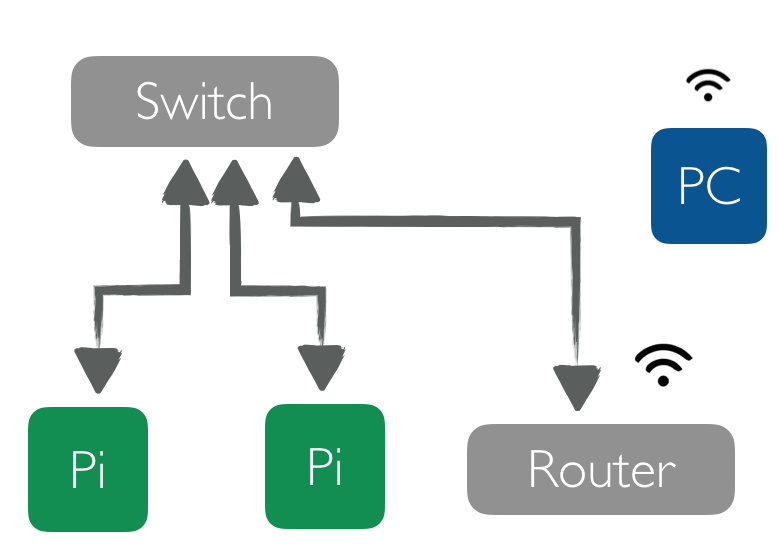
\includegraphics[scale=0.6]{images/tb-temp.png}
	\caption{Testbed setup for temperature sensing flow.}
	\label{fig:tb-temp}
\end{figure} 

\noindent The experiment was tested 8 times and each time  we measured the delay between publishing the flow from the PC $ t_{PC}$ until it is received and deployed by  node-RED instances on the Raspberry Pis $t_{Pi}$, we also measured the delay between flow deployment and the first database temperature insert query on each device's instance $t_{db}$. 
\begin{table}[H]
	\centering
	\begin{tabular}{c|c|c|c|c}\toprule
		&  $ t_{Pi1} - t_{PC}$   & $t_{db} - t_{Pi1}$  & $ t_{Pi2} - t_{PC}$ &  $t_{db2} - t_{Pi2}$ \\ \midrule
$ \overline{t} $ &2.870&	1.723&	2.437&	1.717\\
$ \sigma t $& 0.769	&0.0376&	1.003&	0.013\\
	\end{tabular}
	\caption{Mean and standard deviation of temperature flow delays.}
	\label{table:temp}
\end{table}

\noindent Given these delays, the average time the temperature flow takes to reach the Raspberry Pi and gets deployed is 2.653 seconds which the mean of the two Raspberry Pi delays. The average time from the flow deployment  until the first temperature measurement is inserted in the database    is 1.720 seconds. Which means that in our proof-of-concept implementation, it takes on average 4.373 seconds from the moment 
the temperature flow is deployed until the first database  insertion is done. Given the testbed setup and that the flow does not have large size dependencies, the time should have been less although we think that the Raspberry Pi  low performance capabilities increases the delays and this can be seen in the next experiments  In this experiment we have satisfied some of the requirements mentioned in  Section \ref{sec:requirements}: i) service discovery, ii) send and deploy computations, iii) computation dependencies, iv) pervasiveness.

\section{Recognizing Water Bottles } \label{sec:rwb}


Moving on to more complex scenarios, this use case  is as follows: movements are detected around low computation devices portrayed as the Raspberry Pis. Once they detect movements around them, they take an image and send it to the topic \textit{NUC}. A high performance machine "an Intel NUC" should be waiting for input on the same topic. As soon as the NUC  receives an image, it runs an image recognition algorithm which is a flow itself and responds back to the Raspberry Pi which sent the original message  only if the recognizer recognizes a water bottle. When a Raspberry Pi receives the recognition result on its endpoint, this means that the image was a water bottle with a certain confidence, therefore, the Pi signals a red LED to light up and stores the result in a database. \\ 

\noindent The flow implementation used to create this use case can be found in Sections \ref{subsec:tensor} and \ref{subsec:detect-move}.  As part of this experiment when a flow requiring high amount of performance such as the image recognition flow is received by low performing devices they will not get deployed and  will log that requirements were not satisfied. The same case applies when a flow requiring low amount of computing power is received by a high performing device, of course, this could be optimized because clearly high performance devices can execute flows which are not needy. The computational requirements needed by each flow are decided before sending the flow over to other devices using the HTML page implemented in the publishing flow explained in \ref{subsec:send-comp}.\\ 

This scenario helps us validate several requirements for the framework evaluation: 
\begin{enumerate}
	
	\item Service discovery, through discovering all devices running SCAMPI.
	\item Send and deploy flows, by sending them to all devices connected to a network  running our framework stack and controlling which devices can deploy the flows by sending meta-data for the resources and computation power along with flow. Therefore, being able to only send to some sets of nodes.
	%\item Checking requirements of flows and rejecting the deployment if they were not satisfied at the receiving devices.
	\item Global Identifier, by sending data  to a  specific device using its global identifier.

	\item Computation Dependencies, through carrying tensorflow image recognition and the motion flow dependencies in order to guarantee a successful run at the receiving device.

	\item Communication, by having publish-subscribe messages between the NUC and the Raspberry Pis.
	
	
	\item Pervasiveness, through lighting a red LED once an image bottle is successfully recognized and a message is sent back to the Raspberry Pi.

\end{enumerate}

\noindent As stated every device must have the framework stack running before we start our use case. So after making sure its running we start publishing the flows. In this use case, the testbed setup is shown in Figure \ref{fig:tb-tensor}, it consists of two Raspberry Pis, an Intel NUC and a router connected via switch. The PC which will publish the computations is connected through the router via WI-FI. 
 \begin{figure}[H]
	\centering
	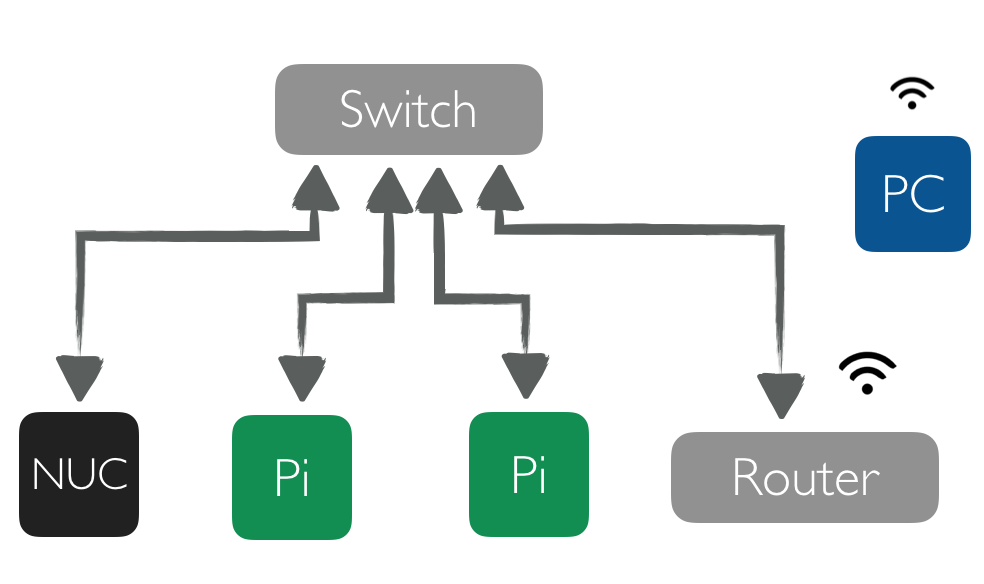
\includegraphics[scale=0.6]{images/tb-tensor.png}
	\caption{Testbed setup for recognizing water bottles.}
	\label{fig:tb-tensor}
\end{figure} 



\noindent We started by publishing the flow \ref{subsec:tensor} for  image recognition with all its dependencies in total 83MB, then we published the motion detection flow \ref{subsec:detect-move} with the sensor scripts. We measured the delay between publishing flows from the PC till it was received and deployed by node-RED on each instance. The use case was tested 8 times, we also measured the delay when a motion was detected by Raspberry Pi and an image was sent to the NUC and the recognizer reply, this was also tested 8 times for each Pi, a total of 16 tests. The sequence diagram displayed in \ref{fig:sd-tensor},  illustrates the procedure in addition to the time initials for each part of the process.  \\



\begin{figure}[H]
	\centering
	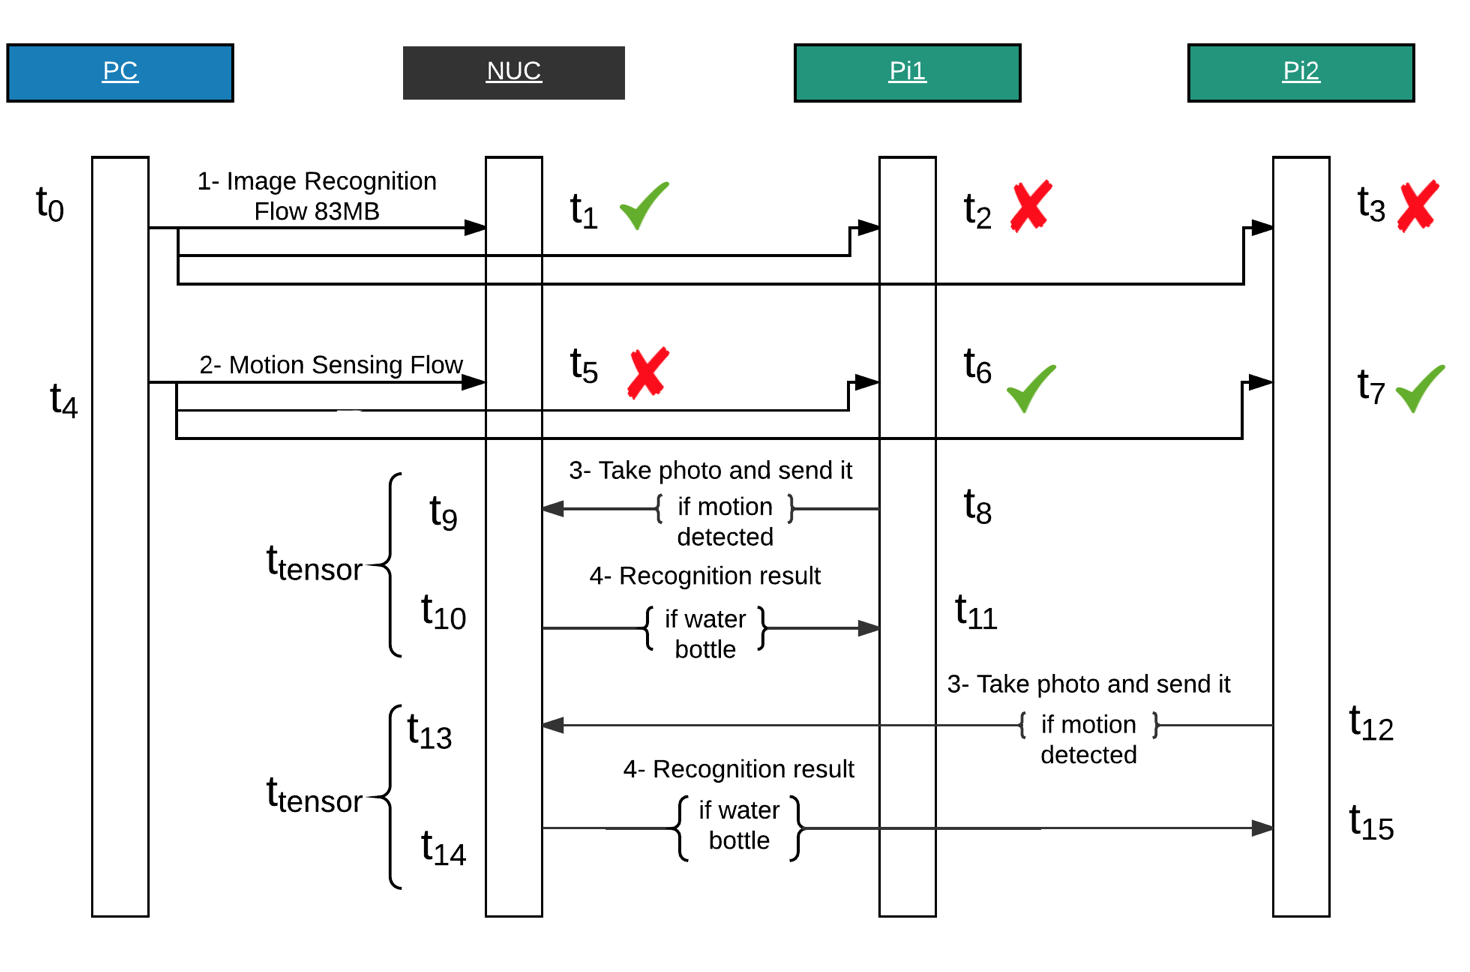
\includegraphics[scale=0.6]{images/sequence-diagram.png}
	\caption{Sequence diagram for recognizing water bottles.}
	\label{fig:sd-tensor}
\end{figure} 
 


\noindent At time $t_0$ the image recognition flow was published, at times $t_1, t_2$ and   $t_3$ it was received by the NUC, Pi1 and Pi2 respectively. The check mark shows that the flow was deployed and the cross mark means deployment was refused because of insufficient resources Then at time $t_4$ the motion sensing flow was published and at times $t_5,t_6$ and $ßt_7$ it was received by the other devices as well. A times $t_8$ and $t_{12}$  the Pis detected motion, took an image and then sent a message to the NUC. At times $t_9$ and $t_{13}$,  NUC received messages from the Pis and started processing, detected a watter bottle and then sent the  results back to the senders at $t_{10}$ and $t_{14}$. The Pis received recognition responses with the confidence percentage at $t_{11}$ and $t_{12}$.  The tables \ref{table:tensor}, \ref{table:motion} and \ref{table:data} show the mean and standard deviation of the delays.  
\begin{table}[H]
\centering
\begin{tabular}{c|c|c|c}\toprule
&$t_1 - t_0$  & $t_2 - t_0$  & $t_3-t_0$ \\ \midrule
$ \overline{t} $&	23.245 s&28.226 s&20.826 s\\ 
$ \sigma t $ &1.440 s&8.830 s&8.851 s\\
\end{tabular}
\caption{Mean and standard deviation of the image recognition flow delays.}
\label{table:tensor}
\end{table}


\begin{table}[H]
\centering
\begin{tabular}{c|c|c|c}\toprule
&$t_5 - t_4$  & $t_6 - t_4$  & $t_7-t_4$ \\ \midrule
$ \overline{t} $ &0.087 s&2.322 s&1.948 s\\
$ \sigma t $&0.012 s&0.053 s&0.491 s\\
\end{tabular}
\caption{Mean and standard deviation of the motion detection flow delays.}
\label{table:motion}
\end{table}

\begin{table}[H]
\centering
\begin{tabular}{c|c|c|c|c|c}	\toprule
&$t_9 - t_8$  & $t_{11} - t_{10}$  & $t_{13}-t_{12}$ & $t_{15}-t_{14}$&  $t_{tensor}$ \\ \midrule
$ \overline{t} $&0.282 s&0.700 s&	0.273 s&0.6985 s&5.512 s\\
$ \sigma t $&0.061 s&0.067 s&	0.048 s&0.0488 s&0.217 s\\
	\end{tabular}
	\caption{Mean and standard deviation for sending and receiving data delays.}
	\label{table:data}
\end{table}

\begin{table}[H]
	\centering
	\begin{tabular}{c|c|c|}	\toprule
		&$t_{11} - t_8$  & $t_{15} - t_{12}$ \\ \midrule
		$ \overline{t} $&6.566 s&	6.592 s\\
		$ \sigma t $&0.097 s&	0.093 s\\
	\end{tabular}
	\caption{Mean and standard deviation for the whole data exchange period delays.}
	\label{table:total}
\end{table}


\noindent It is apparent that delays of the flow carrying image recognition dependencies took long times compared to the motion flow and the data messages between the NUC and Pis. That is mostly because the size of data in which the message is carrying. The data messages included images with size that range  between 50K to 90K  and the motion sensing flow had dependencies with sizes less than 2K. It is also clear that when the receiving side are the Raspberry Pis, delays are usually larger than when the receiving side is the NUC. This is evident in the motion sensing delays in Tables \ref{table:motion} and  also in \ref{table:data} despite that the message sent from the Raspberry Pis to the NUC are heavier   in terms of size than their replies, but the delays are much less. We can also conclude that it takes almost 1 second to have a successful data communication carrying dependencies between the Raspberry Pi and the NUC in our framework, by deducting the time taken in the image recognition process which is on average 5.5 seconds shown in Table \ref{table:data}  from the total time taken to exchange data between the Pi and the  NUC displayed in Table \ref{table:total}.

\section{Local Composability}
In order to prove that we can compose flows locally using our framework, we created a use case that builds on the  previous experiment. Our goal is to use the same database configuration in both flows, one to write into a database while the other reads. Therefore, being able to compose two flows in order to achieve a bigger use case.
\begin{figure}[H]
	\centering
	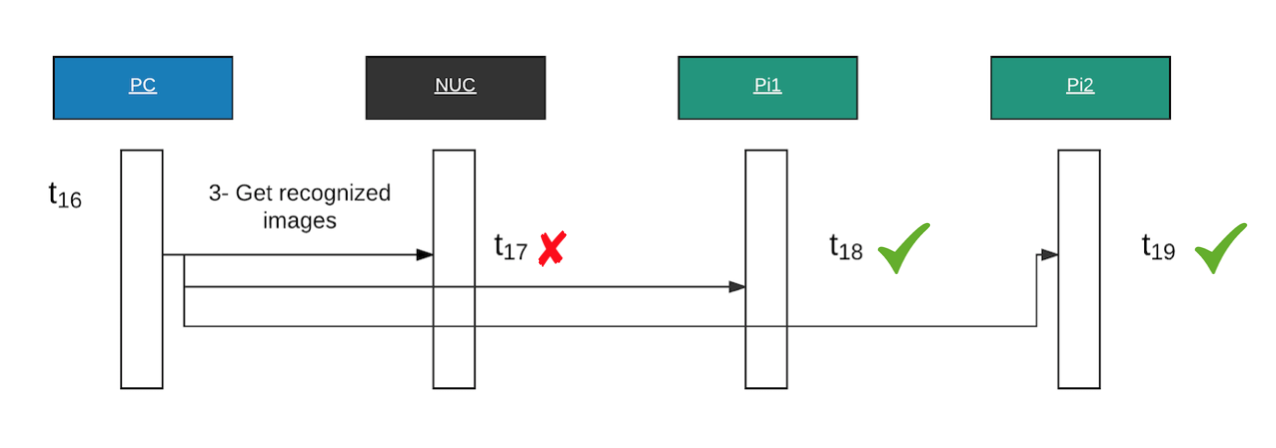
\includegraphics[scale=0.6]{images/sequence-diagram-2.png}
	\caption{Sequence diagram  extension for getting recognized water bottles.}
	\label{fig:sd-images}
\end{figure} 

 \noindent Continuing on the same testbed setup as Section \ref{sec:rwb} and the same scenario.  After the Raspberry Pis stored the recognized images of water bottles into their respective  databases, we sent a flow that retrieves these images from the database into a web endpoint along with their confidence percentages as explained in \ref{subsec:images}.  We retrieved some of the images displayed in  Figure \ref{fig:water-bottles} from the  Raspberry Pi endpoint to prove that the local composability flow works as expected. By doing this, we make sure that flows can be locally composed using the same database configuration. We also measured the delay between sending the flow from the PC until it was deployed by node-RED on other devices. The flow required low computational effort, therefore, it was not  deployed on the NUC device. The experiment was also tested 8 times.

\begin{table}[H]
	\centering
	\begin{tabular}{ c | c | c| c }	\toprule
		&$t_{17} - t_{16}$  & $t_{18} - t_{16}$  & $t_{19}-t_{16}$ \\ \midrule
		$ \overline{t} $&	0.105&	0.801&	0.834\\
		$ \sigma t $&	0.028&	0.060&	0.051\\
	\end{tabular}
	\caption{Mean and standard deviation for retrieving recognized images flow delays.}
	\label{table:images}
\end{table}


\begin{figure}[H]
	\centering
	\begin{tabular}{cc}
		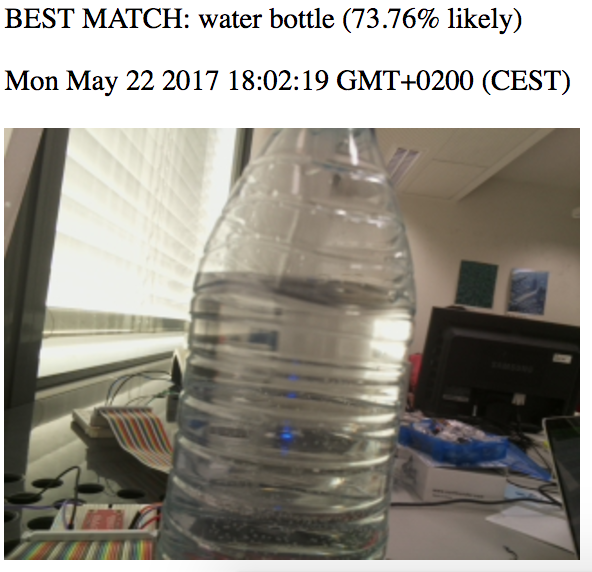
\includegraphics[scale=0.5]{images/water-bottle-1.png}
		&
		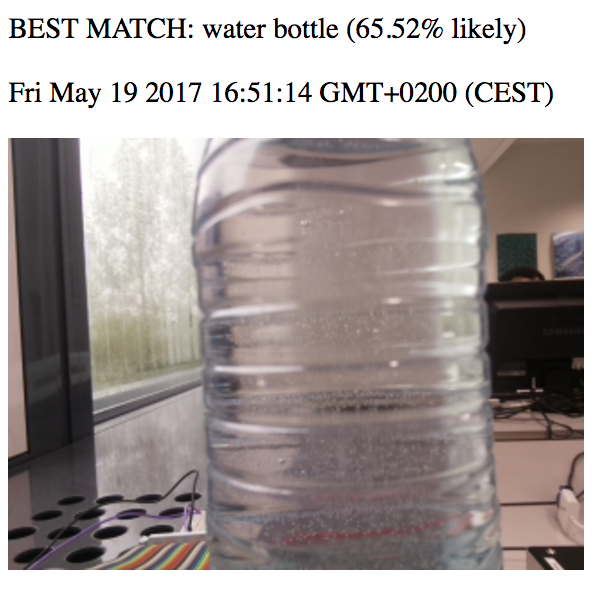
\includegraphics[scale=0.5]{images/water-bottle-2.png}
		\\
		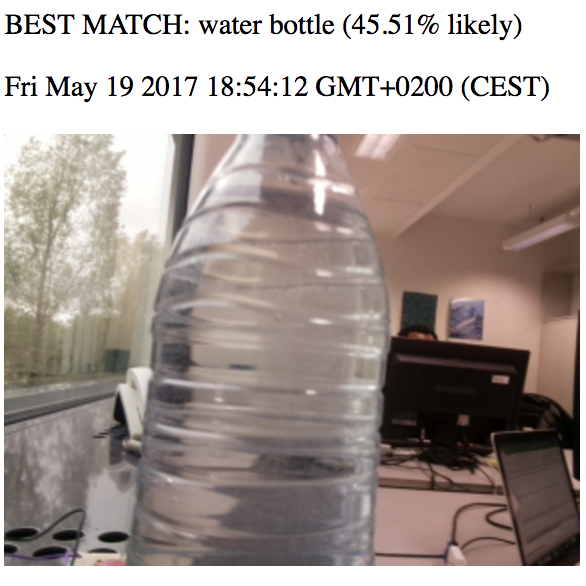
\includegraphics[scale=0.5]{images/water-bottle-3.png}
		&
		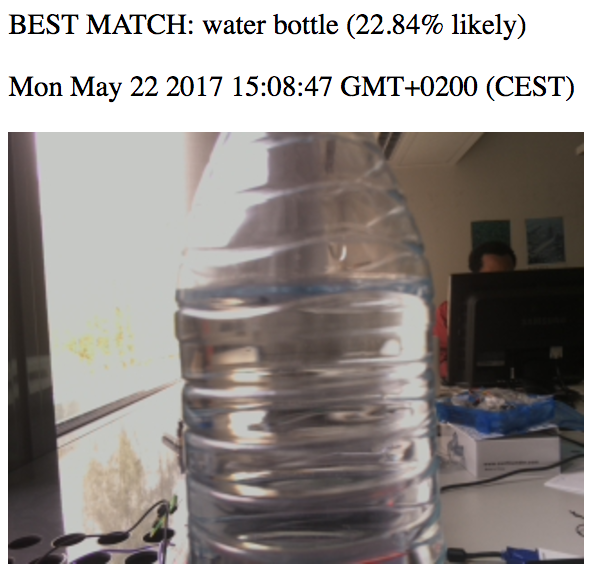
\includegraphics[scale=0.5]{images/water-bottle-4.png}
	\end{tabular}
	\caption{Images of the water bottles received from the NUC.}
	\label{fig:water-bottles}
\end{figure}




\noindent Closer inspection shows that  delays in this use case are quite low because this flow does not have any dependencies at all. Comparing the times in which the Raspberry Pis have received and deployed flows, this one  has quite the least delay. However, the NUC in this flow seemed to have a bit higher delay average than the motion sensing flow with not so much dependencies as well.


\section{Challenged Networks}
The section below shows our aim to evaluate that the framework works in challenged networks with no end-to-end path between  sender and receiver. We used the same setup as \ref{sec:rwb} but with two major changes. The first change is that we disconnected  a Raspberry PI from the network switch, therefore, it is no longer connected to the other devices or the publishing PC, we also set up the disconnected node as an access point in which other devices can connect to using Wi-Fi. The second change is that we introduced an Android phone that can connect to both the Raspberry Pi's access point and the router's Wi-Fi connected to the switch. Additionally, the device exchanges  its Wi-Fi connection between the access point and router Wi-Fi each 80 seconds. The system setup is demonstrated in Figure \ref{fig:tb-dtn}.
\begin{figure}[H]
	\centering
	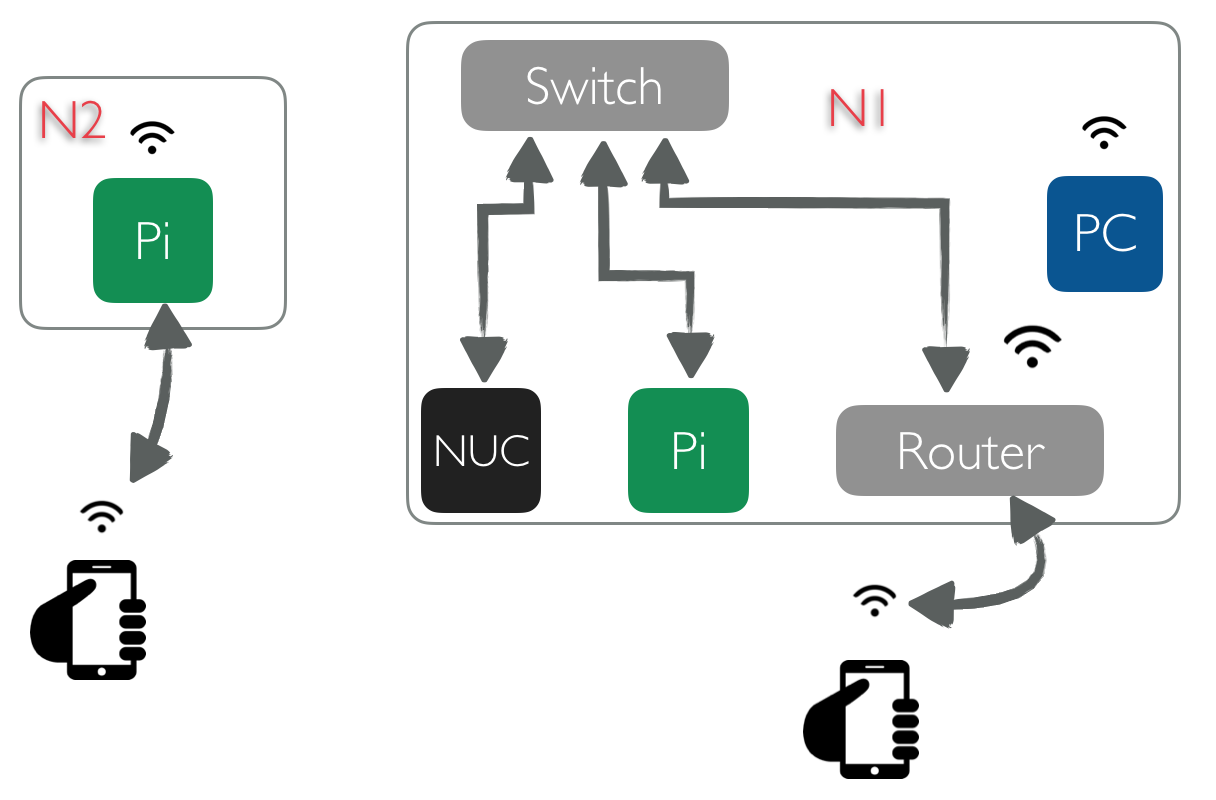
\includegraphics[scale=0.6]{images/tb-dtn.png}
	\caption{Testbed setup for challenged and delay tolerant networks.}
	\label{fig:tb-dtn}
\end{figure} 

\noindent The experiment was tested only one time for an extended amount of 50 minutes. First, we used the PC to publish the image recognition flow and the motion sensing flow. Second, we waited some time until we made sure that the flows have reached the disconnected Pi. Afterwards, we passed hands over the infrared sensor of the disconnected Pi and put a water bottle in front of the camera. We repeated this action multiple times.\\

\noindent This use case is evaluated differently, since in the current Maestro implementation, we do not have a way to map requests sent to with their respective responses. In the experiment explained in Section \ref{sec:rwb}, each request was only sent once hence we received only one response, however this is not the case here. Since we sent more than one request at once and not all of them were recognized as  water bottles, therefore there was no response from the NUC for these requests. Thats why we evaluate this use case on 3 different levels. First, the delay between publishing  flows from the PC and receiving them on all devices. Second, the delay between sending the images from the disconnected Pi to the NUC. Third, the delay between sending the results from NUC till they are deployed to the disconnected Pi.  Take into account that, the number of messages sent from the Pi to the NUC and vice versa may not be equal due to the fact that some images were not recognized as water bottles. In addition, we have no means to map a message which was sent as an image recognition request to another one sent as a response which could be an enhancement to Maestro. \\

\noindent The following table shows the first evaluation phase, $t_{NUC}$, $t_{Pi}$ and $t_{disconnected-pi}$ are the delays between publishing the flows from the PC till it reaches each device.
\begin{table}[H]
	\centering
	\begin{tabular}{c|c|c|c}\toprule
		&$t_{NUC}$  & $t_{Pi1}$  & $t_{disconnected-pi}$ \\ \midrule
		image recognition flow& 39.414&	53.719&	312.072s\\
		motion sensing flow&3.163&	5.401&	215.657\\
	\end{tabular}
	\caption{The delays for sending flows to the network devices including the disconnected PI.}
	\label{table:DIS}
\end{table}

\noindent From the above table we can definitely see the delay added to the disconnected Pi. This main reason for that  is, beside not having a direct connection, the switching window of the Android device. It can affect the transfer in different ways. If the switching time is too big, the delay will most probably increase because after a flow is uploaded to the phone, it will have to wait for some time until the window closes before it switches back to the other network. But also, having it too small, flows with  large size of dependencies will not succeed to upload their data to the Android phone in time. \\


\noindent Next we show the delays of some messages that were sent from the disconnected Pi to the NUC carrying images with their average and standard deviation.
\begin{table}[H]
	\centering
\begin{tabular}{c|c}\toprule
		  & $t$  \\ \midrule

$ \overline{t} $&	185.818\\
$ \sigma t $&	54.966\\
\end{tabular}
	\caption{Delay mean and standard deviation of 13 messages sent from the disconnected Raspberry Pi to the NUC.}
	\label{table:DIS2}
\end{table}

\noindent Finally, we evaluated the response message returning back from the NUC to the disconnected Raspberry Pi having successfully recognized a water bottle.

\begin{table}[H]
	\centering
	\begin{tabular}{c|c}\toprule
		& $t$  \\ \midrule
$ \overline{t} $& 	90.467\\
$ \sigma t $&	59.770\\
	\end{tabular}
	\caption{Delay mean and standard deviation of 10 messages sent from the NUC to disconnected Raspberry Pi having successfully recognized water bottles.}
	\label{table:DIS3}
\end{table}


\noindent What stands out in the previous tables is that delays are much bigger, but the good thing is that several devices were able to communicate despite not having any direct connection between each other. We were also able to deploy computations to a device which was not in our publishing network.

\begin{figure}[H]
	\centering
	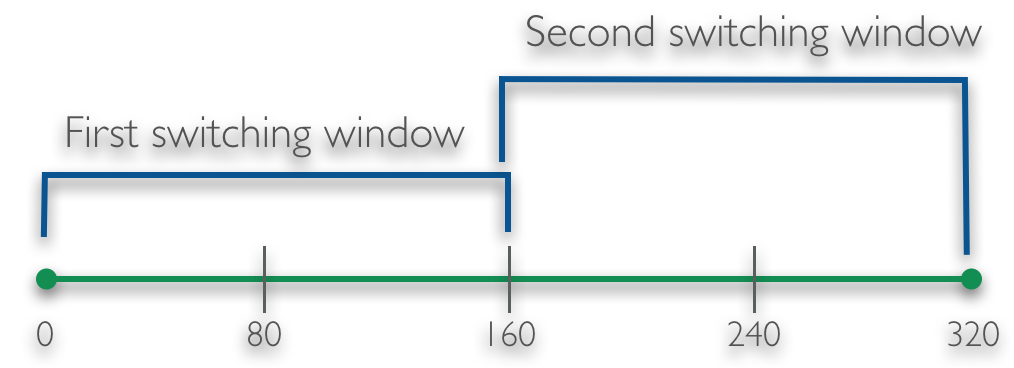
\includegraphics[scale=0.6]{images/switch.png}
	\caption{Timeline for the Android device switching process.}
	\label{fig:window}
\end{figure} 


 \noindent When the messages are sent or the flows are published, we do not know whether the android device is connected to the sender at that point or not, thats why we evaluate the delay time according to the whole transfer window which is 160 seconds as demonstrated in \ref{fig:window}.  We think that the average delay in Table \ref{table:DIS3}  for delivering responses which is  90.467 seconds is acceptable.  Since it means that the transfer was done in the first switching window. Further, The average times  of the flows and messages sent from the Pi to the NUC in Tables  \ref{table:DIS} and \ref{table:DIS2}  are also acceptable. Being from 160 to 320 seconds means that it had to wait for the second switching window which makes sense  because these messages were carrying images, scripts and libraries as dependencies .
\section{Summary}

During this chapter, we have distributed our framework and middleware implementation evaluation on several parts each describing a different use case with various requirements. We started by showing the typical IoT usage of sensor networks in which we deployed a computation that monitors temperature on several devices.  Then, we went on with a more complex scenario where we ran image recognition algorithm on high performing machines which received messages from devices with low computation capabilities. Afterwards, we showed how flows can be composed locally using the same database configuration. Finally, we created a delay-tolerant network with a disconnected device and showed that we can deploy computations and communicate with the disconnected devices.
